\documentclass[a4paper]{article}
%\documentclass[8pt]{report}
%%%%%%%% CREATE DOCUMENT STRUCTURE %%%%%%%%
%% Language and font encodings
\usepackage[english]{babel}
\usepackage[utf8x]{inputenc}
\usepackage[T1]{fontenc}

%\usepackage{subfig}

%% Sets page size and margins
\usepackage[a4paper,top=3cm,bottom=2cm,left=2cm,right=2cm,marginparwidth=1.75cm]{geometry}

%% Useful packages
\usepackage{amsmath}
\usepackage{graphicx}
\usepackage[colorinlistoftodos]{todonotes}
\usepackage[colorlinks=true, allcolors=blue]{hyperref}
%\usepackage{caption}
\usepackage[justification=centering]{caption}
\usepackage{subcaption}
\usepackage{sectsty}
\usepackage{float}
\usepackage{titling} 
\usepackage{blindtext}
\usepackage[square,sort,comma,numbers]{natbib}
\usepackage[colorinlistoftodos]{todonotes}
\usepackage{xcolor}
\usepackage{fancyhdr}
\usepackage{lipsum}

%% definitions 
\definecolor{darkgreen}{rgb}{0.0, 0.4, 0.0}

%% Define your personal info here %%%%%%%%%%%%%%%%%%%%%%%
\newcommand\TPid{5}
\newcommand\TPname{Network Learning Using PSO}
\newcommand\Firstname{Joao Filipe}
\newcommand\Familyname{Costa da Quinta}
\newcommand\Email{Joao.Costa@etu.unige.ch}

%%%%%%%%%%%%%%%%%%%%%%%%%%%%%%%%%%%%%%%%%%%%%%%%%%%%%%%

%%%%%%% Page header %%%%%%
\pagestyle{fancy}
\fancyhf{}
\rhead{TP \TPid: \TPname}
\lhead{\Firstname \Familyname}
\rfoot{Page \thepage}


%%%%%%%% DOCUMENT %%%%%%%%
\begin{document}

%%%% Title Page
\begin{titlepage}

\newcommand{\HRule}{\rule{\linewidth}{0.5mm}} 							% horizontal line and its thickness

\center 
 
% University
\textsc{\LARGE Université de Genève}\\[1cm]

% Document info
\textsc{\Large Metaheuristics for optimization}\\[0.2cm]									% Course Code
\HRule \\[0.8cm]
{ \huge \bfseries TP \TPid : \TPname}\\[0.7cm]								% Assignment
\HRule \\[2cm]
\large
\emph{Author:} \Firstname \; \Familyname\\[0.5cm]		
\emph{E-mail:} {\color{blue}\Email}\\[7cm]		
% Author info
% Author info
{\large \today}\\[2cm]

\includegraphics[width=0.4\textwidth]{images/unige_csd.png}\\[1cm] 	% University logo
\vfill 
\end{titlepage}


% ============================================
% ----------------------------------
\newpage
\section{Introduction}
During this TP we will be working with Artificial Neural Networks (NN) to try and classify images, there will be two labels, either the image contains the number 2, or it doesn't. Neural Networks attempt to mimic the general way that actual biological neurons work. This is done by connecting the output single Neurons that have $[0,1]$ as possible outputs, as input to other single Neurons. Each unique neuron can give its output to many different Neurons, and receive as input the output of many neurons. At the final layer we will have only 1 neuron that outputs $\{0,1\}$.\\\\ We will implement a NN that has 3 layers, the first layer has 400 neurons, the second has 25, and the third has 1 neuron. A neuron from any given layer receives its input from neurons that are in the previous layer, and gives its output to neurons in the next layer. The first layer receives as input the numerical value of a single pixel from the image, since the images are all 20x20 there are 400 unique pixels, one for each neuron from the first layer. The first and second layer contain an offset Neuron that receive no input, and output the value $1$, which means the final numbers are 401 neurons for the first layer and 26 for the second.

\section{Particle Swarm Optimization}
Particle Swarm Optimization (PSO) is an algorithm that like the Ant System, trusts that the group is capable of a better answer than a single individual. But rather than communicating only though a complex system, here individuals will share their best results with all the other individuals. Then at each iteration, each individual will make a decision about their next step, basing themselves on their own trajectory, their own personal best, and the group overall best result. 
\section{Particle Swarm Optimization for Neural Networks}
As explained previously, each neuron receives a certain number of inputs from other neurons. To transform all the different inputs into a single output, each neuron must compute different values, so that it is able to perform a weighted sum of all the inputs. These weights are the values that we will try to optimize so that we can label as many as possible images correctly. This might seem somewhat complex, but it is actually very easy once we visualize it, the following image will help with that:

\begin{figure}[H]
\center
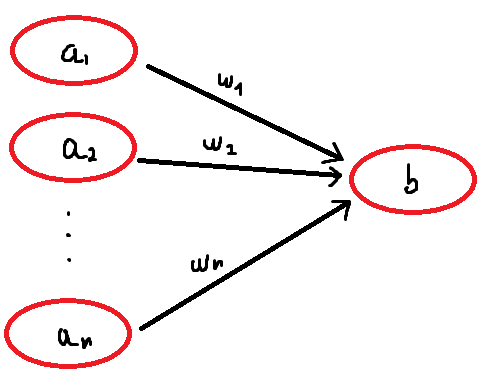
\includegraphics[width=0.5\textwidth]{images/neurons_f.PNG}
\caption{Neuron b, receives as input the values from neurons $\{a_1,a_2, ..., a_n\}$, neuron's b value is computed by:\\ $b = a_1 * w_1 + a_2 * w_2 + ... + a_n * w_n$}
\end{figure}

Now lets see how the algorithm works:
\begin{itemize}
\item[(1)] define the number of particles (individuals), and the number of iterations, we will later see how these affect the results
\item[(2)] for each particle initialize the all weights randomly between the following interval [-0.5, 0.5], as well as its velocity set to 0
\item[(3)] for each particle compute its error with the random initialized weights, compare the result to best result found by the same particle, update it if necessary
\item[(4)] compute the global best result
\item[(5)] for each particle compute the new velocity by using the following formula:\\
$$v_{t+1} = w v_{t} + c_1 r_1(b_t - s_t) + c_2 r_2(B_t - s_t)$$\\
$w, c_1, c_2$ are predefined constants, $= 0.9, 2, 2$ respectively\\
$r_1, r_2$ are random values between [0,1)\\
$b_t, B_t$ are the best solution found by the particle at iteration t, and the global best solution at iteration t\\
$s_t$ is the current position of the particle
\item[(6)] for each particle update its position by using the following formula:\\
$$s_{t+1} = s_t + v_{t+1}$$
\item[(7)] go back to step (3) -> a given number of times, which is defined in step (1)
\item[(8)] return global best solution
\end{itemize}

Let's talk the search space, our initial vector v is of size 401x1, which means that to turn it into a vector of 25 values (one for each neuron of the second layer) we need to do a matrix multiplication where the second matrix is of size 25x401, this matrix represents the weights (every neuron of the second layer receives the value from every neuron of the first layer). Next we do the same between the second and third layer.\\\\
We have the multiplication between first and second layer : $v_1 = W_1 v, v_1$ is of size 25x1\\
And a second multiplication between the second and third layer : $v_2 = W_2 v_1, v_2 $ is of size 1x1\\
$W_1$ is of size 25x400, and $w_2$ is of size 1x26, since each weigh is bound by the interval [-0.5, 0.5], the dimension of the search space is $[-0.5,0.5]^{25*400+26}$.\\
After each matrix multiplication we apply the sigmoid function, that mimics the threshold of a neuron passing an impulse in the brain.
\newpage
\section{Results}
I found that more particles would make the system converge faster, rather than more iterations. So for our initial results, there were 20 particles, and 10 iterations.

\begin{figure}[H]
\center
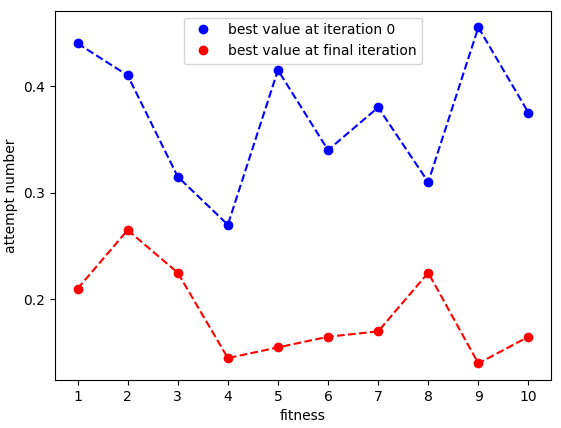
\includegraphics[width=0.8\textwidth]{images/best_fit.PNG}
\caption{Best value ant iteration 0 and best value at final iteration}
\end{figure}
With this plot we can see that the best value at the first iteration doesn't influence the best value at the end of the last iteration.

\begin{figure}[H]
\center
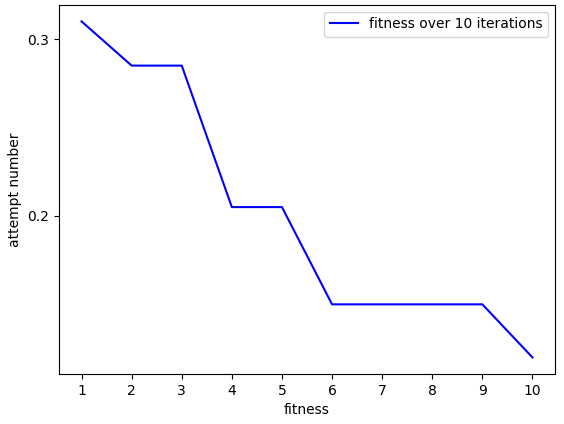
\includegraphics[width=0.8\textwidth]{images/fit_over_10.PNG}
\caption{Best fitness over 10 iterations}
\end{figure}
We can see the fitness slowly converging to 0, however, at around the iteration 8, it usually reaches its minimum.

\begin{figure}[H]
\center
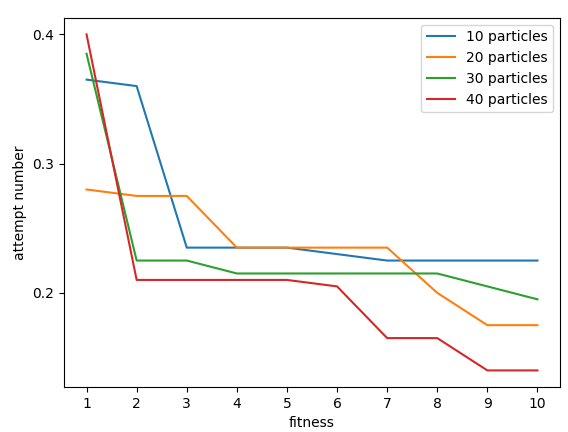
\includegraphics[width=0.8\textwidth]{images/fit_over_particles.PNG}
\caption{fitness over 10 iterations for different numbers of particles}
\end{figure}
As expected, increasing the number of particles will most likely improve the best solution, but it is obviously more costly in time and memory

\begin{figure}[H]
\center
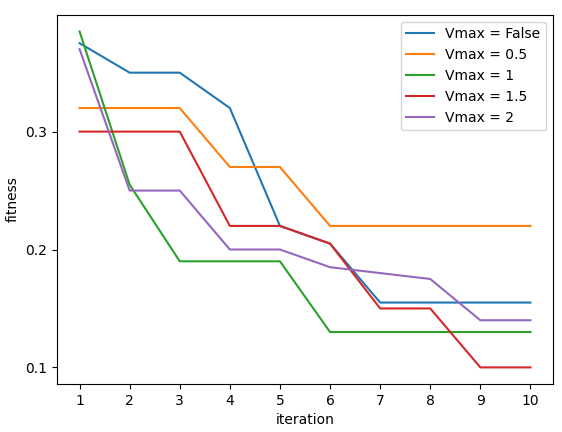
\includegraphics[width=0.8\textwidth]{images/v_max.PNG}
\caption{fitness over 10 iterations for different values of Vmax}
\end{figure}
Setting a cut-off value makes it so the fitness converge faster!
\end{document}
